%%%%%%%%%%%%%%%%%%%%%%%%%%%%%%%%%%%
\subsection{Front-end Readout \& Buffering}
\label{sec:fd-daq-fero}

\metainfo{Giles Barr \& Giovanna Miotto \& Brett Viren, this is DP-specific.  This file is \texttt{far-detector-dual-phase/chapter-fddp-daq/design-fero.tex}}

\begin{dunefigure}[DP front-End DAQ fragment]{fig:daq-readout-buffering-baseline}
  {Illustration of data (solid arrows) and trigger (dashed) flow for
    one DP front-end DAQ fragment. 
    Black arrows indicate nominal flow and red indicate special flow
    for handling of potential SNB.  See text for detail description.}
  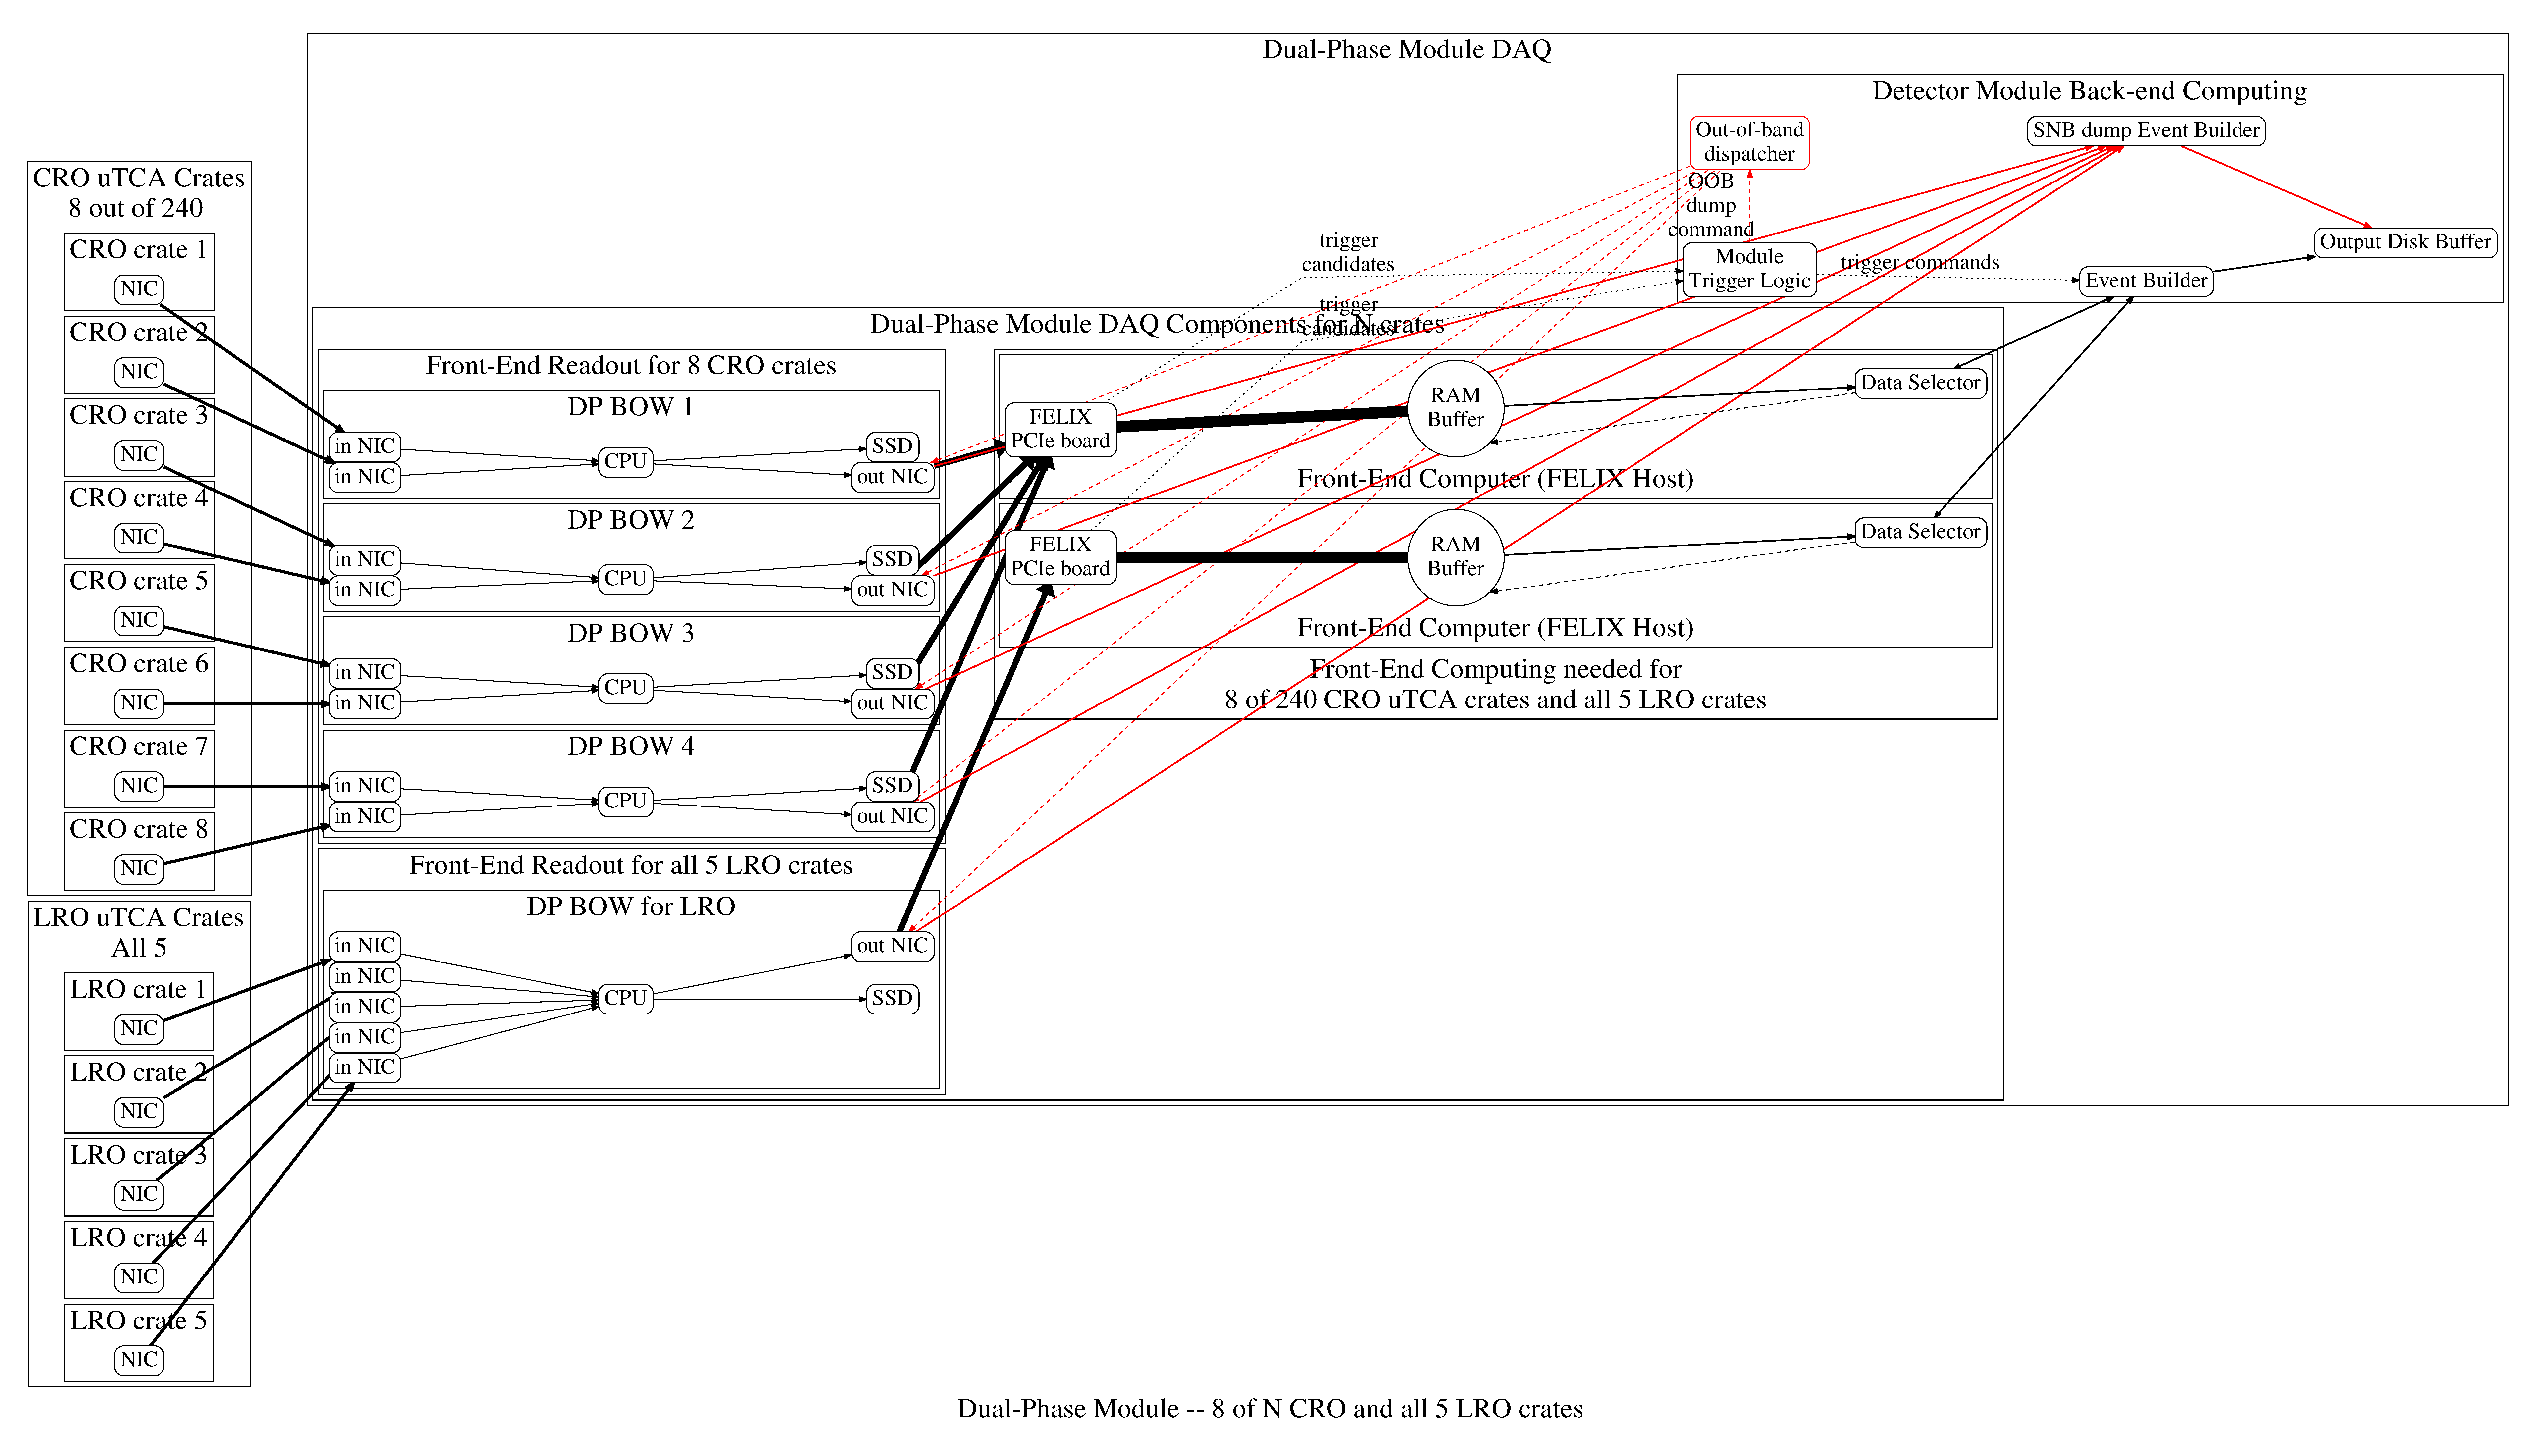
\includegraphics[width=0.8\textwidth]{daq-readout-buffering-baseline.pdf}%
\end{dunefigure}

Figure~\ref{fig:daq-readout-buffering-baseline} illustrates
DP-specific implementation of the nominal, generic DAQ front-end
\dword{daqfrag} design shown in Fig~\ref{fig:daq-overview}. 
The CRO crates deliver data on UDP to ``bump on wire'' (BOW) computers
which implement the \dword{daqfer} duties.
The CRO data is delivered to the DAQ BOW computers with lossless
compression applied and so before the \dwords{trigprimitive} can be
produced the data must be decompressed. 

In order to save on cost, power, space, cooling, etc, a number of CRO
crate data streams can be aggregated into one \dword{fec}. 
The CRO data stream is sent using UDP which is not expected to provide
reliable transport of high throughput data if a network switch
intervenes. 
Thus each CRO requires a corresponding 10 Gbps NIC in the receiving
BOW computer.
With the expected 10$\times$ lossless compression factor the nominal
output from each CRO crate will be 2 Gbps. 
If noise levels are higher than expected the throughput will increase
however even very noisy data should be compressible enough to fit into
the 10 Gbps bandwidth. 
Noise will be better understood from ProtoDUNE-DP data and studies
will be needed in order to optimize the number of CRO crates per BOW
computer.

After processing, the input data is sent out, along with the
corresponding primitives to a FELIX board in a \dword{fec}. 
Similar to the argument above about noise, bandwidth and BOW computer
multiplicity, the number of BOW data streams that can be aggregated
into each FELIX board requires additional study. 
The current generation of FELIX boards have been tested to with a
throughput to system RAM of \SI{10}{\GB/\s}. 
The next generation is expected to at least double that. 
With the caveat that these tests did not receive data on UDP a nominal
\SI{20}{\GB/\s} throughput is assumed possible for the next generation
PCIe v4 boards. 
Given this assumption and that the expected noise levels are achieved
then based solely on bandwidth as many as 80 CRO data streams might be
aggregated into a single next-generation FELIX board. 
Figure~\ref{fig:daq-readout-buffering-baseline} indicates the
aggregation of eight CRO stream which represents the multiplicity
required to deal with very high noise. 
Future studies are needed to understand which of these two extremes
the design may be optimized toward but the basic design itself is
fairly elastic between them.

The LRO crates are nominally not involved in self-triggering although
their data are considered to flow through a LRO BOW. 
This includes data from all five LRO crates which is then sent to a
single FELIX board. 
Given their expected data rates, that FELIX board must ingest about
\SI{25}{\GB/\s}.

The second duty of the \dword{daqfer} in the nominal design is to
provide non-volatile storage for receiving full-stream data dumps when
a \dword{snb} dump trigger command is issued. 
With today's technology, individual SSDs can write at about 2.5 GB/s. 
Up to four SSDs have been placed on a 16 lane PCIe v3 board and have
achieved about three times this. 
This would allow an individual BOW computer to aggregate 10 to 30 CRO
data streams before the SSDs become a bottleneck. 
The five LRO data streams, each producing 5 Gbps, could together be
streamed to a two modern SSDs. 
The BOW computers must also have sufficient RAM to hold
pre-SNB-trigger data of about 10 seconds.

The alternative design (not diagrammed) which corresponds to
Fig~\ref{fig:daq-overview-alt} deletes the layer containing BOW
computers and directly connects the UDP streams from the CRO and LRO
crates to the FELIX boards in the \dwords{fec}. 
The CRO (compressed) data is buffered on the FELIX host computer ram
and distributed to the trigger farm for decompression and trigger
primitive and trigger candidate processing. 
The remaining part of the \dword{trigdecision} is as in the nominal
design except that the SNB dump data stream is handled symmetrically
with the normal triggered data.
